\section{Dataset}
\label{sec:data}

Hierarchical datasets are rare~\cite{bade_creating_2008}.

\subsection{Reuters Dataset}


\subsection{Banksearch Dataset}

We obtained the dataset from Carnegie Mellon University~\footnote{\url{http://lib.stat.cmu.edu/datasets/} (29.12.2025)}.
Like \cite{bade_creating_2008}, we use the complete structure of the banksearch dataset but subsample 100 samples per category.
We employ this dataset to directly compare our work to existing approaches.


\begin{figure}[h]
\centering
\resizebox{0.5\linewidth}{!}{%
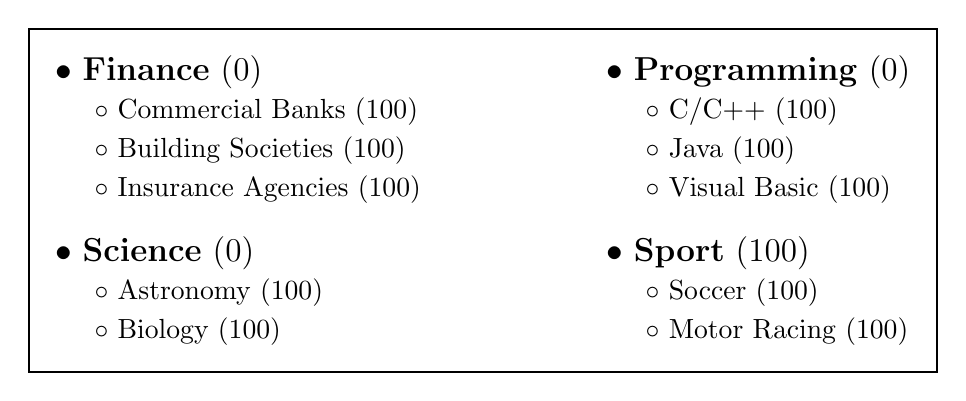
\begin{tikzpicture}[baseline=(current bounding box.north)]
  \usetikzlibrary{fit}

  % Left column
  \node (f1) [anchor=west] at (0.5,5.5) {\large$\bullet$ \textbf{Finance} (0)};
  \node (f2) [anchor=west] at (1.0,5.0) {$\circ$ Commercial Banks (100)};
  \node (f3) [anchor=west] at (1.0,4.5) {$\circ$ Building Societies (100)};
  \node (f4) [anchor=west] at (1.0,4.0) {$\circ$ Insurance Agencies (100)};

  \node (s1) [anchor=west] at (0.5,3.2) {\large$\bullet$ \textbf{Science} (0)};
  \node (s2) [anchor=west] at (1.0,2.7) {$\circ$ Astronomy (100)};
  \node (s3) [anchor=west] at (1.0,2.2) {$\circ$ Biology (100)};

  % Right column
  \node (p1) [anchor=west] at (7.5,5.5) {\large$\bullet$ \textbf{Programming} (0)};
  \node (p2) [anchor=west] at (8.0,5.0) {$\circ$ C/C++ (100)};
  \node (p3) [anchor=west] at (8.0,4.5) {$\circ$ Java (100)};
  \node (p4) [anchor=west] at (8.0,4.0) {$\circ$ Visual Basic (100)};

  \node (sp1) [anchor=west] at (7.5,3.2) {\large$\bullet$ \textbf{Sport} (100)};
  \node (sp2) [anchor=west] at (8.0,2.7) {$\circ$ Soccer (100)};
  \node (sp3) [anchor=west] at (8.0,2.2) {$\circ$ Motor Racing (100)};

  % Dynamic outer box (this replaces the fixed rectangle)
  \node[
    draw,
    line width=0.8pt,
    fit=(f1)(s3)(p1)(sp3),
    inner sep=6pt
  ] {};
\end{tikzpicture}%
}
\caption{Banksearch dataset \cite{bade_creating_2008}.}
\end{figure}



